\documentclass{standalone}
\usepackage{tikz}
\begin{document}
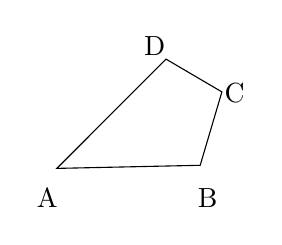
\begin{tikzpicture}[x=1pt,y=1pt]
\draw (83.40,-124.98) -- (135.20,-123.86) -- (143.05,-97.34) -- (122.87,-85.50) -- cycle;
\node at (79.95,-135.75) {A};
\node at (137.95,-135.75) {B};
\node at (147.62,-97.78) {C};
\node at (118.77,-80.88) {D};
\end{tikzpicture}
\end{document}
